\section{Verification Approach}
%figures : 
We give a basic outline of our proof of our correctness theorem.

We want to show that $\mathtt{execute\_tree\_list} (tree\_list) \in error\_states$.

We prove this by first proving Theorem \ref{thm:etl}.

\begin{proof}[Theorem \ref{thm:etl}]
This is a proof by induction on the size of $tree\_list$.

For our base case we show that if $tree\_list$ is of length $1$, then $\mathtt{execute\_tree\_list} (tree\_list) \in \mathtt{concretize\_leaf} (t)$.


To prove this we use the following set property (which we verify in Coq):

\begin{theorem}
$\forall$ inputs $i$,
If $A \in B$ and 
$\forall x \in B$, \concexecution($x, i$) $\in C$, then  \concexecution($A, i$) $\in$ $C$.
\label{thm:set2}
\end{theorem}

If $tree\_list$ is of length $1$, we know we are executing from the initial concrete state of the system. Therefore, we consider the following properties:
\begin{itemize}
\item $init\_conc\_state \in 
  \mathtt{concretize\_root} (\mathtt{last\_element} (tree\_list))$. (Property $1$)
 \item $ \forall$ inputs $i$, 
 $\forall x \in
  \mathtt{concretize\_root} (\mathtt{last\_element} (tree\_list))$,  
 $ \concexecution(x, i) \in \mathtt{concretize\_leaf}(\mathtt{last\_element}(tree\_list))$.
\end{itemize}

Now, using Theorem \ref{thm:set2}, we conclude that $\concexecution(init\_conc\_state) \in \mathtt{concretize\_leaf}(\mathtt{last\_element}(tree\_list))$.

Our inductive hypothesis is  $\mathtt{execute\_tree\_list} (tree\_list') \in \mathtt{concretize\_leaf} (\mathtt{last\_element}(tree\_list'))$ where $tree\_list'$ is $tree\_list$ with the last element removed.

We want to show that if our inductive hypothesis holds, then $\mathtt{execute\_tree\_list} (tree\_list) \in \mathtt{concretize\_leaf}(tree\_list)$.

In order to prove this, we must prove the following lemma:
\begin{lemma} 
\label{lem:etl}
$\mathtt{execute\_tree\_list} (tree\_list') \in \mathtt{concretize\_root} (\mathtt{last\_element} (tree\_list))$.
\end{lemma}
\begin{proof}[Lemma \ref{lem:etl}]
We prove this using the following set property (which we verify in Coq):

\begin{theorem} \label{thm:set1}
If $A \in B$ and $B \subseteq C$, then $A \in C$.
\end{theorem}

We know:
\begin{itemize}
\item$ \mathtt{execute\_tree\_list}(tree\_list') \in
        \mathtt{concretize\_leaf} (\mathtt{last\_element}(tree\_list')) $. (Inductive Hypothesis)
\item 
$\mathtt{concretize\_leaf} (\mathtt{last\_element}(tree\_list')) \subseteq \mathtt{concretize\_root} (\mathtt{last\_element} (tree\_list))$. (Property $3$)
 \end{itemize}
 
 So, using Theorem \ref{thm:set1}, we conclude that $\mathtt{execute\_tree\_list} (tree\_list') \in \mathtt{concretize\_root} (\mathtt{last\_element} (tree\_list))$. \qed
\end{proof}

Now, to prove our inductive step, we know:
\begin{itemize}
\item $\mathtt{execute\_tree\_list} (tree\_list') \in \mathtt{concretize\_leaf} (\mathtt{last\_element}(tree\_list'))$. (Lemma \ref{lem:etl})
\item if $x \in \mathtt{concretize\_root}(\mathtt{last\_element}(tree\_list))$, then  $\concexecution(x, get\_input (l.\pathcondition)) \in \mathtt{concretize\_leaf}(\mathtt{last\_element}(tree\_list))$,
where $l$ is a leaf of $\mathtt{last\_element}(tree\_list)$. (Lemma \ref{cop})
\item $\mathtt{concretize\_leaf}(t) \neq \{\} $. (Property $3'$)
\end{itemize}

So, using Theorem \ref{thm:set2}, we can conclude that $\mathtt{execute\_tree\_list} (tree\_list) \in \mathtt{concretize\_leaf} (\mathtt{last\_element}(tree\_list))$. \qed
\end{proof}

Now, we prove our correctness property.

\begin{proof}[Theorem \ref{thm:sufficiency}]
We know:
\begin{itemize}
\item $\mathtt{execute\_tree\_list}(tree\_list) \in \mathtt{concretize\_leaf}(\mathtt{last\_element}(tree\_list))$. (Theorem \ref{thm:etl})
\item $\mathtt{concretize\_leaf} (\mathtt{last\_element} (tree\_list)) \subseteq error\_states$. (Property $2'$)
\end{itemize}
so, using Theorem \ref{thm:set1}, we conclude
$\mathtt{execute\_tree\_list} (tree\_list) \in error\_states$. \qed
\end{proof}

The reason we need Property $2'$ is because Property $2$ is not sufficient. This is because if $\mathtt{execute\_tree\_list} (tree\_list) \in \mathtt{concretize\_leaf} (\mathtt{last\_element}(tree\_list))$ and $\mathtt{concretize\_leaf} (\mathtt{last\_element} (tree\_list)) \cap error\_states \neq \{\}$, we could get the case where
$\mathtt{execute\_tree\_list} (tree\_list) \notin error\_states$, as shown in Figure \ref{fig:Prop2}.

\begin{figure}
\label{fig:Prop2}
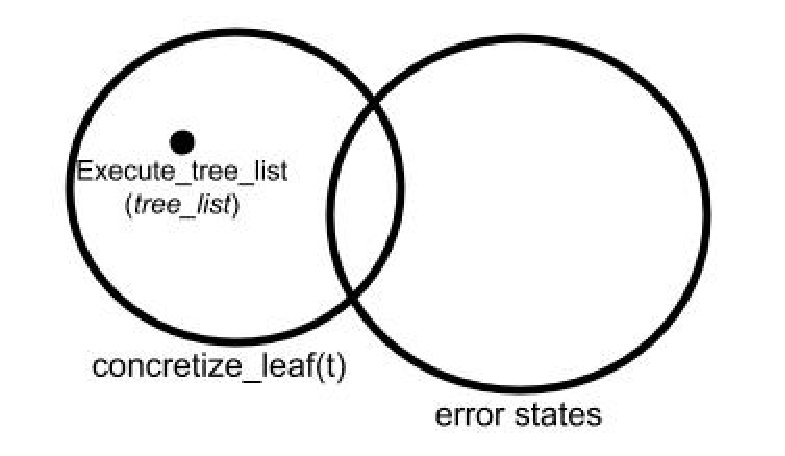
\includegraphics[width=\textwidth]{prop2.eps}
\caption{Example of Property $2$ not being sufficient to show $\mathtt{execute\_tree\_list} (tree\_list) \in error\_states$.}
\end{figure}




